Android is an open-source operating system for mobile devices. The Android project/operating system was initially created by the Open Handset Alliance which includes organizations from various industries such as Google, Vodafone, T-Mobile, LG, Huawei, Asus, Acer, and eBay to give some examples \footnote{\url{http://www.openhandsetalliance.com/oha_members.html}}. To be more specific, Android is an open-source software stack made for a varied range of mobile devices with different structure parameters. The main goal of the Android project is to provide an open software platform accessible for a variety of stakeholders such as developers, engineers, carriers, and device manufacturers to turn their innovative and imaginative ideas into successful real-world products that improve the mobile experience for the end-users. Today, numerous organizations from Open Handset Alliance and also other organizations are supporting and investing in Android and the project is led by Google. Android is designed in a distributed way to avoid the issue of the central point of failure. In another means, different industry players confine or control the advancements of another. As a result, a production-quality consumer product comes along with open source code that is ready for customization.

The platform architecture of Android consists of 6 major layers. Each layer has its own responsibility and handles a different area of the Android operating system. The following figure demonstrates the layers in a way that they are ordered from the highest level of abstraction from the top to the bottom. More detailed information about the Android mobile operating system can be obtained through the official Android documentation \footnote{\url{https://developer.android.com/guide/platform}} \footnote{\url{https://source.android.com/}}.
\begin{figure}
    \centering
    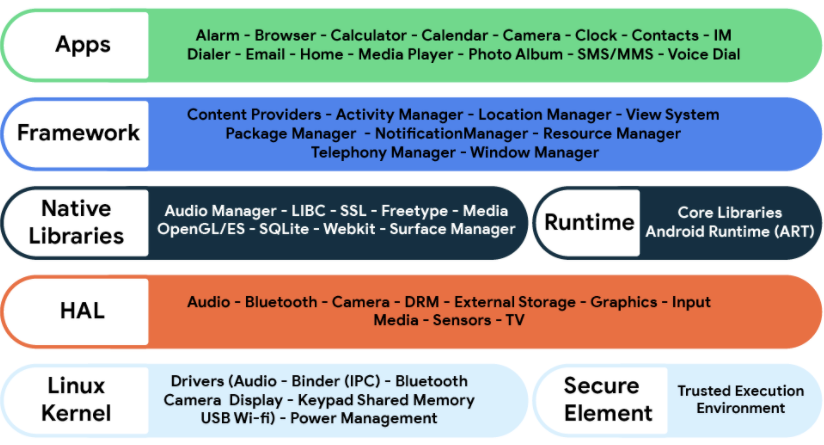
\includegraphics[scale=0.5]{figures/android_os.png}
    \caption{Android platform architecture}
    \label{fig:android_platform_architecture}
\end{figure}

%Upcoming sections give a brief description of each major layer of the Android platform architecture mentioned in Fig. \ref{fig:android_platform_architecture}.